\chapter{Diseño de casos de prueba}
\begin{figure}[htbp]
   \centering
   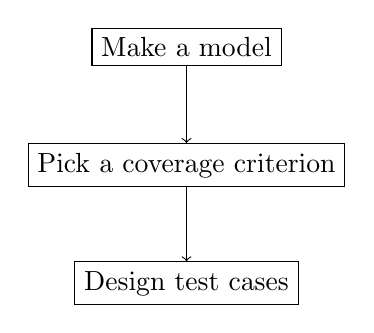
\begin{tikzpicture}[node distance=1.5cm]
      \node (model) [rectangle, draw] {Make a model};
      \node (coverage) [rectangle, draw, below of=model] {Pick a coverage criterion};
      \node (testcases) [rectangle, draw, below of=coverage] {Design test cases};
      
      \draw [->] (model) -- (coverage);
      \draw [->] (coverage) -- (testcases);
   \end{tikzpicture}
\end{figure}

\note{Recuerda que el SUT (System under test) es el sistema bajo prueba.}

Abajo vamos a ver algunos modelos.

\section{Clases de equivalencia}

Se modela el input domain, y para ello se utilizan clases de equivalencia.
Es importante notar que las clases de equivalencia son una asunción, y no una verdad absoluta,  pueden ser erróneas.
\begin{paracol}{2}
   
   \colfill
   Sea $R$ una relación de equivalencia sobre un
   conjunto $A$. Para cada $a \in A$, llamaremos
   clase de equivalencia de $a$, al conjunto
   formado por todos los elementos de $A$ que
   estén relacionados con él a través de $R$.
   \colfill
   
   \switchcolumn

   \begin{figure}[htbp]
      \centering
      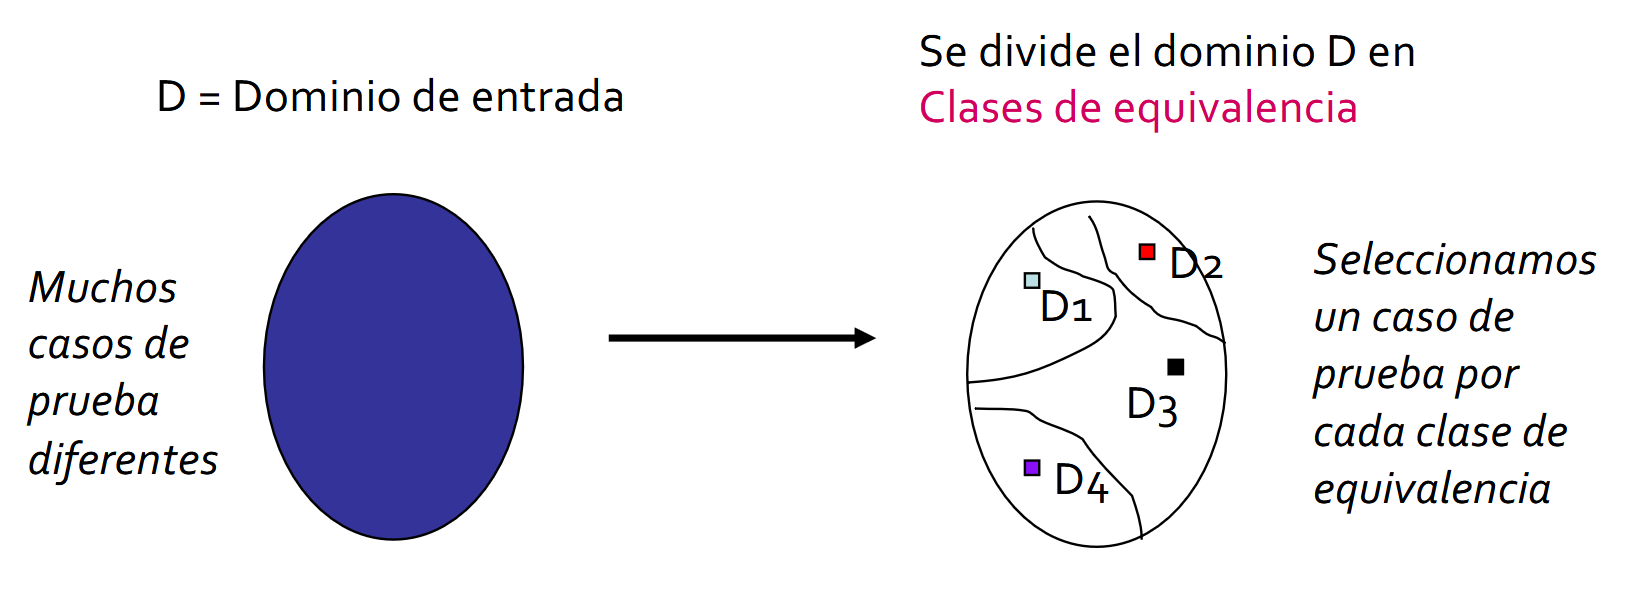
\includegraphics{images/05/claseequivalencia.png}
      \caption{Dividir el dominio}
      \label{fig:05/claseequivalencia}
   \end{figure}
\end{paracol}

Este modelo permite identificar conjuntos de pruebas de tamaño manejable seleccionando unos pocos casos de prueba para cada clase de equivalencia.
Permite también medir la efectividad de la prueba en términos de cobertura relacionada con el modelo de partición creado.
Además, el proceso de partición obliga al tester a pensar sistemáticamente sobre lo que importa.


\newpage
\begin{figure}[htbp]
   \centering
   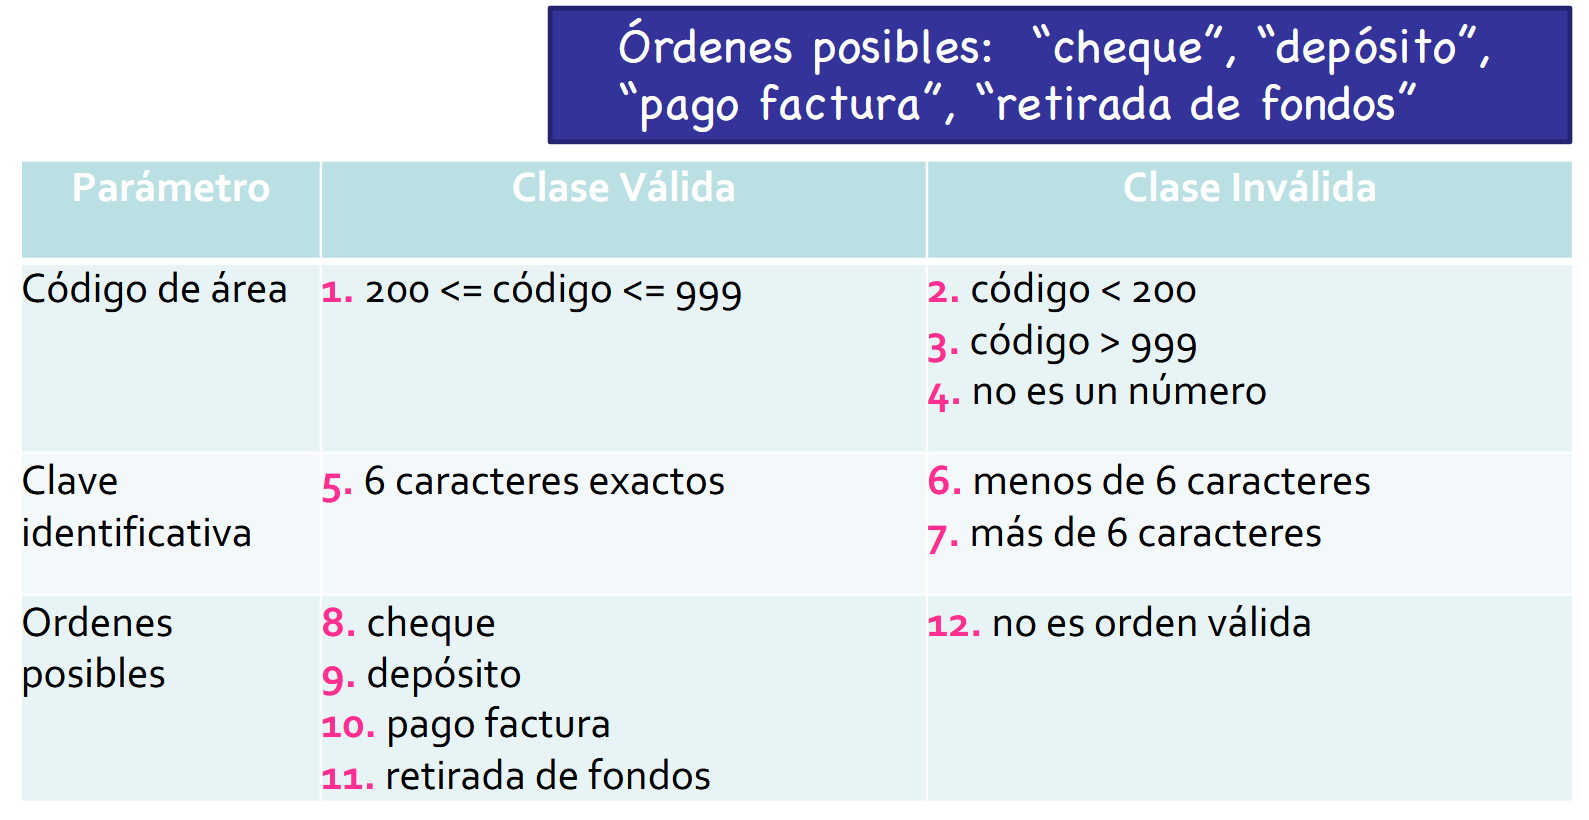
\includegraphics[width=0.65\columnwidth]{images/05/claseBanca.png}
   \caption{Ejemplo de una aplicación bancaria}
   {Los datos de entrada son:\ns
   \begin{itemize}
   	\item Código de area: número de tres dígitos que no empieza ni por 0 ni por 1
	\item Clave identificativa de la operación: 6 caracteres alfanuméricos
	\item Órdenes posibles: ``cheque'', ``depósito'', ``pago factura'' , ``retirada de fondos'' 
   \end{itemize}}
   \label{fig:05/claseBanca}
\end{figure}

Es importante enumerar las clases de equivalencia, y no mezclarlas sobre todo.
Cuando se va a escribir las pruebas, cada prueba tiene que ser relacionada con una o más clases de equivalencia, y tenemos que indicar a cuales.

\begin{table}[htbp]
   \centering
   \begin{tabular}{|c|c|c|}
   \hline
       \textbf{Parámetro} & \textbf{Clase Válida} & \textbf{Clase Inválida} \\ \hline
       Capital & $c > min$ & $c \leq min$ \\ \hline
       Ingreso & $i \geq 0$ & $i < 0$ \\ \hline
       Deuda & $d \geq 0$ & $d < 0$ \\ \hline
       Impagados & $T \vee F$ & \\ \hline
       \multirow{4}{*}{Impagados $\wedge$ cond} & 1) $T \wedge (i - d) < c/3$  & ~ \\
       & 2) $F \wedge (i - d) \geq c/3$ & \\
       & 3) $T \wedge (i - d) \geq c/3$ & \\
       & 4) $F \wedge (i - d) < c/3$ & \\ \hline
   \end{tabular}
   \caption{Ejemplo de clases de equivalencia para una aplicación bancaria}
   \note{
   \begin{itemize}
   	\item si el cliente está en una lista de impagados y el sueldo bruto menos la deuda
   	      es inferior al capital solicitado dividido entre 3, la solicitud pasa a No
   	      Concedida.
   	\item si el cliente no está en ninguna lista, y el sueldo bruto menos la deuda es
   	      mayor o igual al capital solicitado dividido entre 3, se clasifica como Pre-concedida.
   	\item en cualquier otro caso pasa a En estudio
   \end{itemize}
   }
   \label{tab:05/claseEquivalencia}
\end{table}

\subsection{Coverage criterion}
El criterio de cobertura es una forma de medir la efectividad de las pruebas.
{Puede ser:\ns
\begin{itemize}
   \item \textbf{ACoC} - All combinations coverage\\
   para cada variable de entrada se consideran todas las clases válidas, y luego se combinan con todas las clases de las demás variables.
   \item \textbf{ECC} - Each choice coverage\\
   solo se asegura que (un valor de) cada clase ocurra en al menos un caso de prueba
\end{itemize}

Reglas básicas:
\begin{enumerate}
	\item Se pueden combinar valores de clases válidas en el mismo caso de prueba
	\item No se pueden combinar valores de clases inválidas en el mismo caso de prueba. Se necesita un caso de prueba para cada clase inválida
	\item Se debe intentar reducir el número de casos de prueba
\end{enumerate}
}

\begin{figure}[htbp]
   \centering
   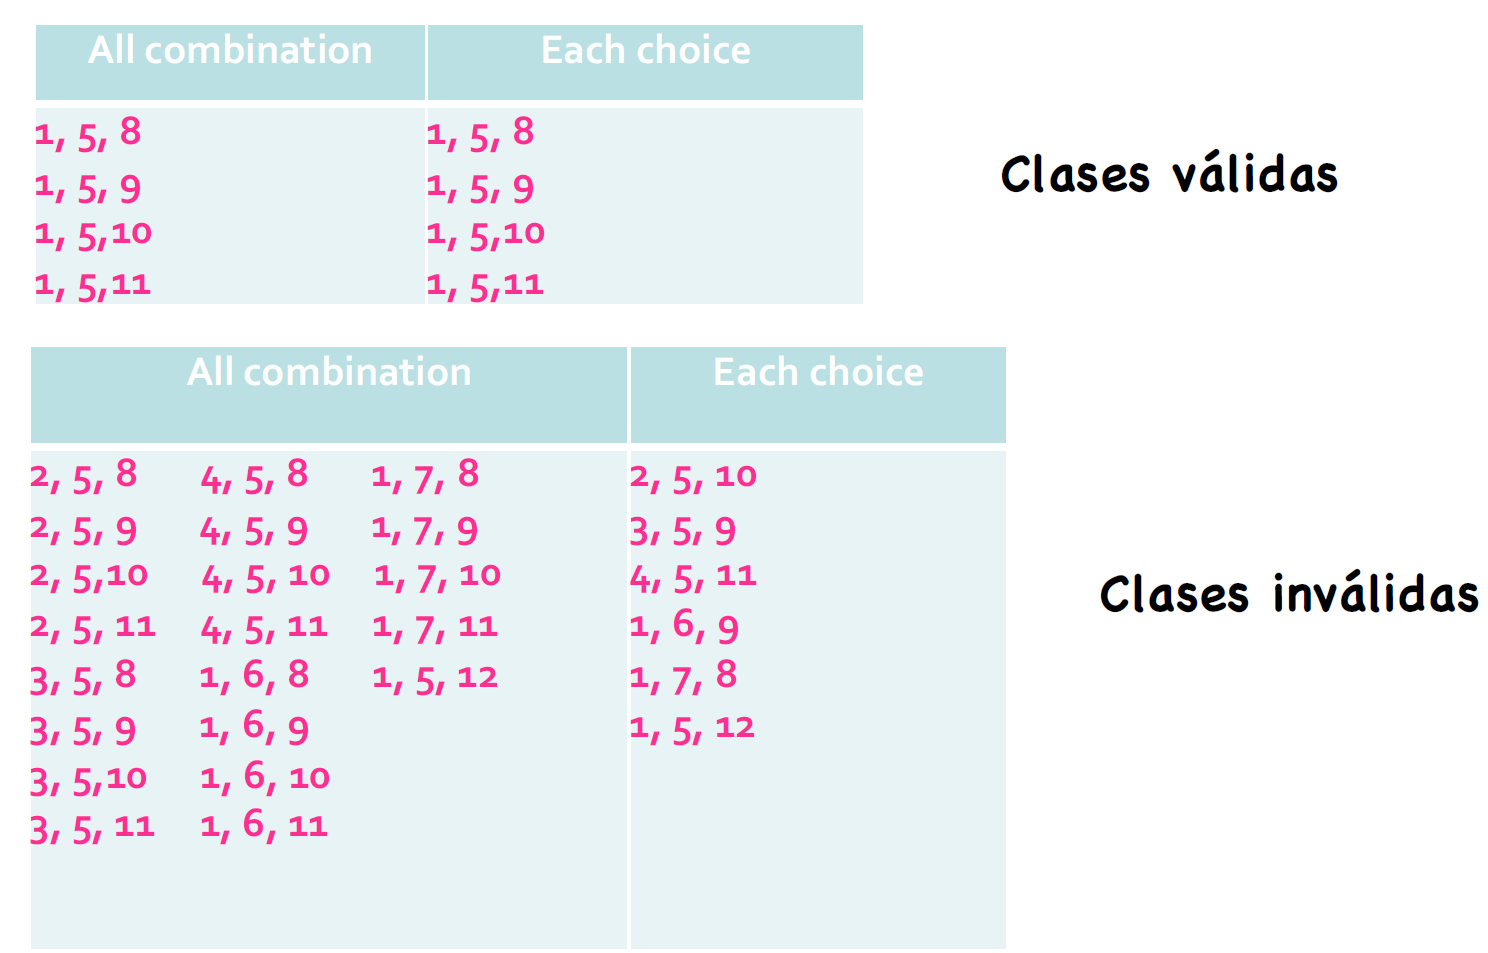
\includegraphics{images/05/criterioCobertura.png}
   \caption{Aplicar los dos criterios de cobertura al ejemplo anterior en Fig. 
   \ref{fig:05/claseBanca}. Aquí se muestran las combinaciones de clases, son tripletas porqué hay tres variables de entrada.}
   \label{fig:05/criterioCobertura}
\end{figure}


\newpage
\section{Design test cases}
\begin{table}[htbp]
   \centering
   \begin{tabular}{|c|c|c|c|}
      \hline
      \textbf{Test case}   & \textbf{Código de area}  & \textbf{Clave identificativa}  & \textbf{Orden}\\ \hline
      \texttt{1,5,8}       & 300             & nómina                & cheque \\ \hline
      \texttt{1,5,9}       & 400             & viajes                & depósito \\ \hline
      \texttt{1,5,10}      & 500             & coches                & pago factura \\ \hline
      \texttt{1,5,11}      & 600             & comida                & retirada de fondos \\ \hline
   \end{tabular}
   \caption{Ejemplo: para cada tripleta que representa una combinación, elegimos un valor que pertenezca a la clase
   de equivalencia.}
   \label{05/testCases}
\end{table}


\section{Tablas de decisión}

Se puede utilizar para programas que toman decisiones basadas en condiciones lógicas sobre combinaciones de entradas, parámetros y/o variables, eligiendo diferentes acciones o respuestas.
\note{\begin{itemize}
	\item La acción o respuesta que se toma no depende del orden en que
se evalúa los valores de los parámetros y variables.
	\item La acción o respuesta que se toma no depende de entradas o
salidas anteriores
\end{itemize}}

\begin{paracol}{2}
   \begin{itemize}
   	\item Cada condición corresponde a una variable, relación o predicado
	\item Valores posibles para las ``Condition Entries''
 \begin{itemize}
 	\item Booleano (\lstinline|True / False|) - Tabla de decisión de entrada limitada
	\item Valores - Tabla de decisión de entrada extendida
	\item Valor ``No Importa'' (Don't care value)

 \end{itemize}
\item Cada acción es una operación que hay que ejecutar

   \end{itemize}
\switchcolumn
\begin{figure}[htbp]
   \centering
   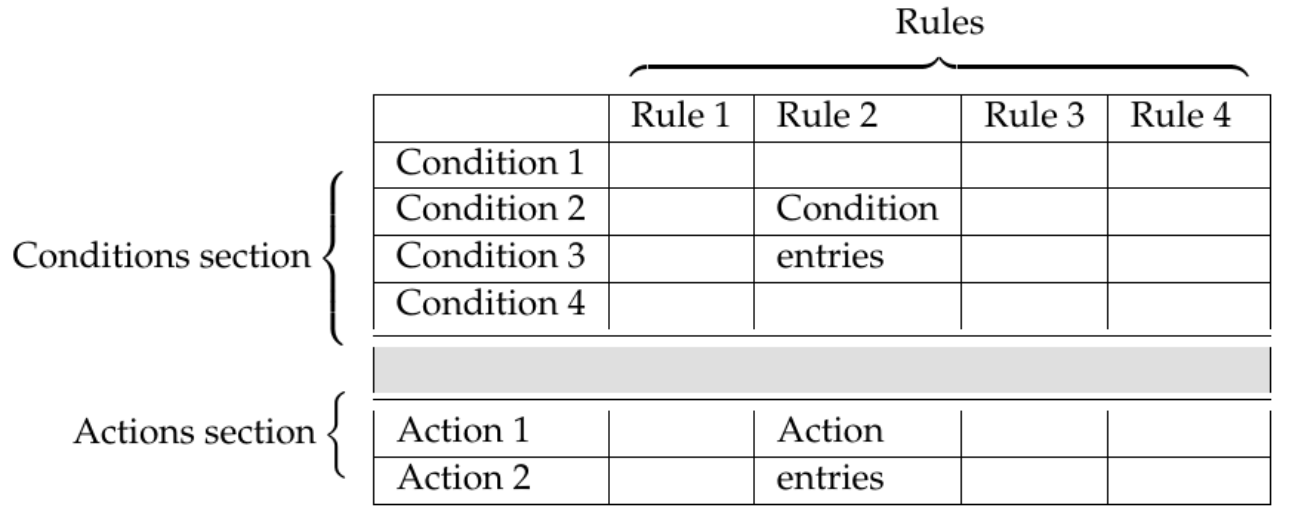
\includegraphics[width=0.99\columnwidth]{images/05/tabladecision.png}
   \caption{Tabla decision }
   \label{fig:05/tabladecision}
\end{figure}
\end{paracol}

\begin{figure}[htbp]
   \centering
   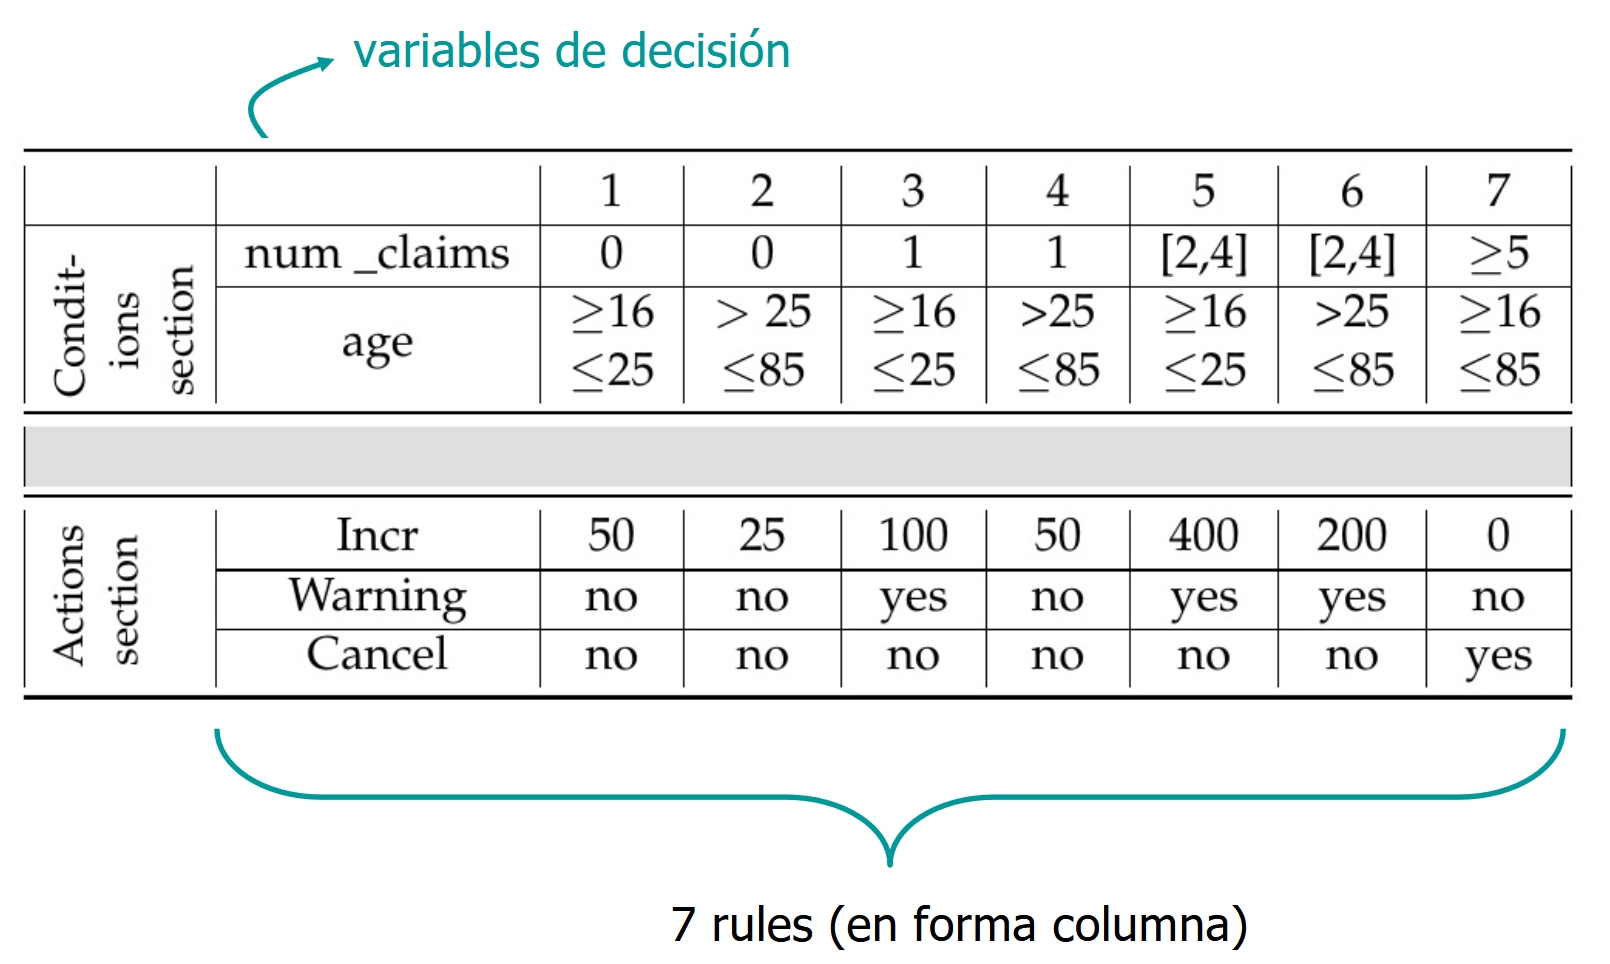
\includegraphics{images/05/tablaForma1.png}
   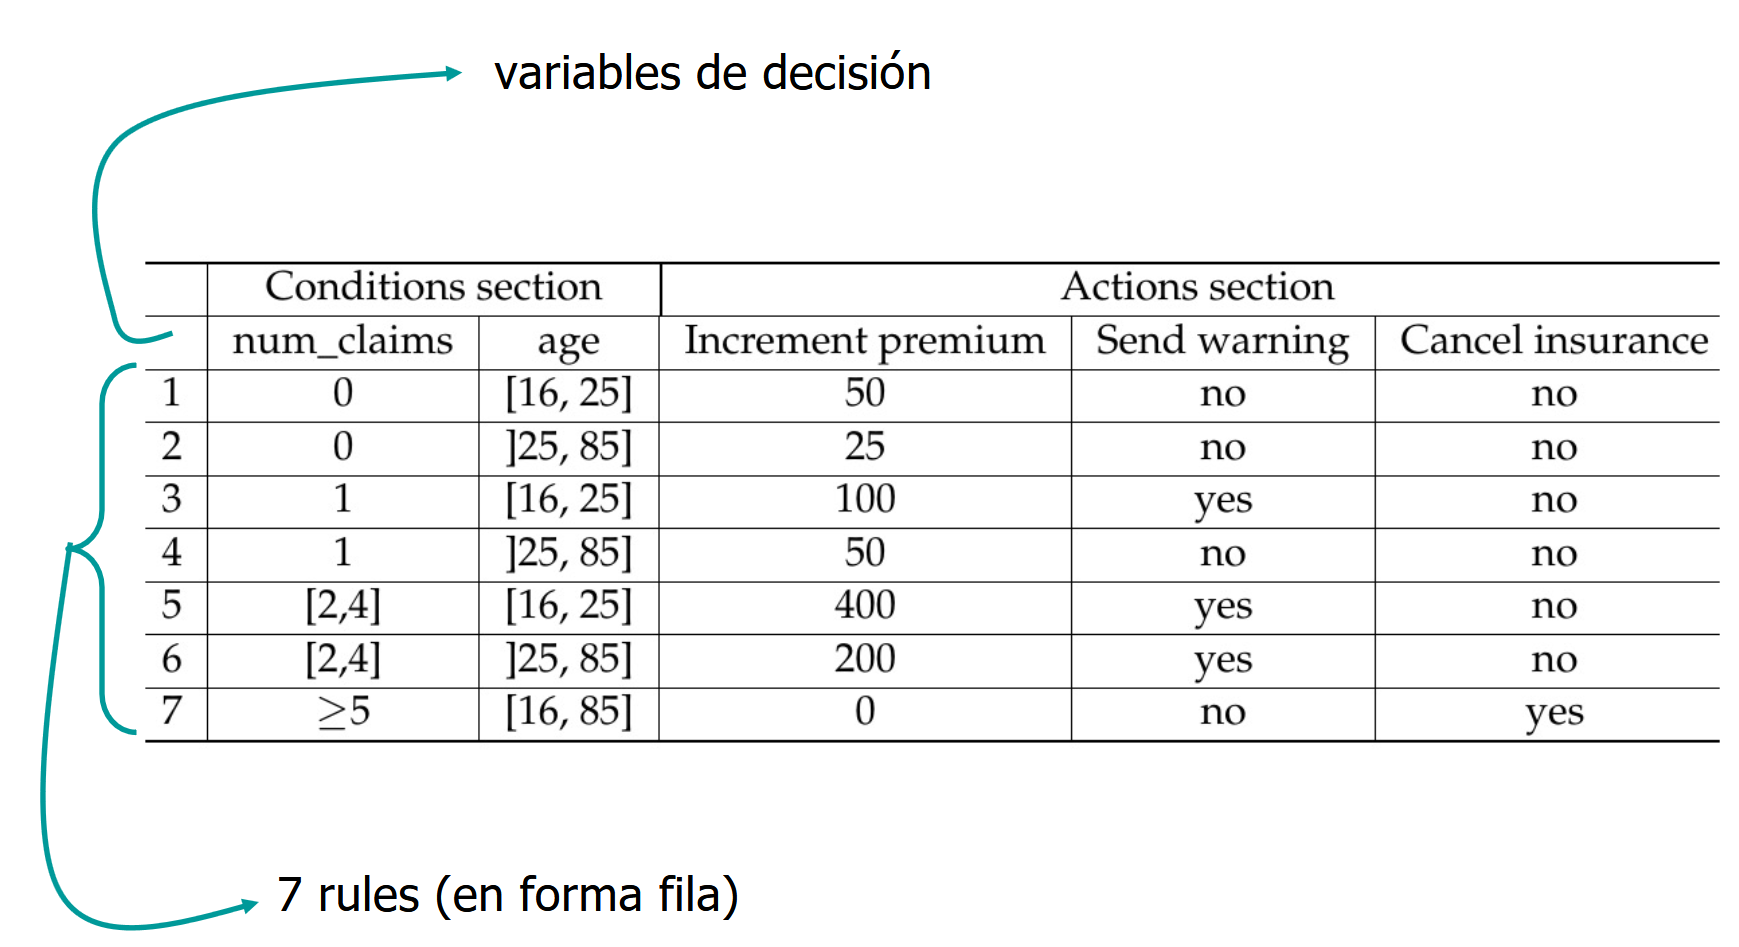
\includegraphics{images/05/tablaForma2.png}
   \caption{Forma columna y forma fila de tablas de decisión}
   \label{fig:05/tablaForma}
\end{figure}

\newpage
\subsection{Criterio de cobertura}
\begin{itemize}
	\item Un caso de test para cada variante explícita
	\item Un caso de test para seleccionar la acción por defecto (si hay)
\end{itemize}

% \newpage

\section{Valores Límites}
La técnica de valores límites es una técnica \textit{complementaria} a las clases de equivalencia y tablas de decisión.
Busca encontrar los errores que se pueden producir en los extremos de los datos de entrada, ya que el sentido común indica que los puntos cercanos a los límites pueden ser más propensos a errores.
\begin{itemize}
	\item \textbf{Intervalo}: un subconjunto del espacio de los valores de entrada de
un programa.
	\item \textbf{Punto límite} de un intervalo (\textit{boundary}): aquel punto que según
sea incrementado o decrementado un valor epsilon infinitesimal
dará como resultado un valor perteneciente o no a dicho intervalo.
	\item \textbf{Desigualdad} del límite: una expresión algebraica con $>$, $<$, $\geq$, $\leq$
que define parte de los puntos que pertenecen a un intervalo o
dominio.
	\item \textbf{Condiciones de igualdad}: una expresión algebraica con $=$, $\neq$
\end{itemize}

\begin{figure}[htbp]
   \centering
   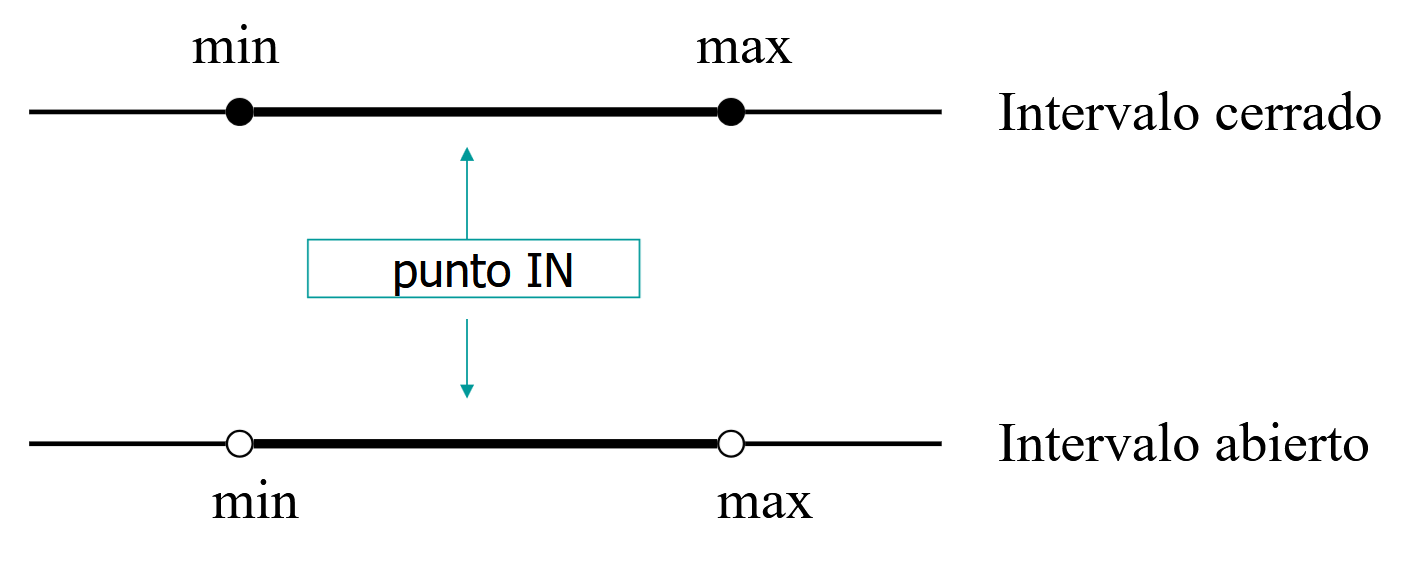
\includegraphics[width=0.45\columnwidth]{images/05/puntoIN.png}
   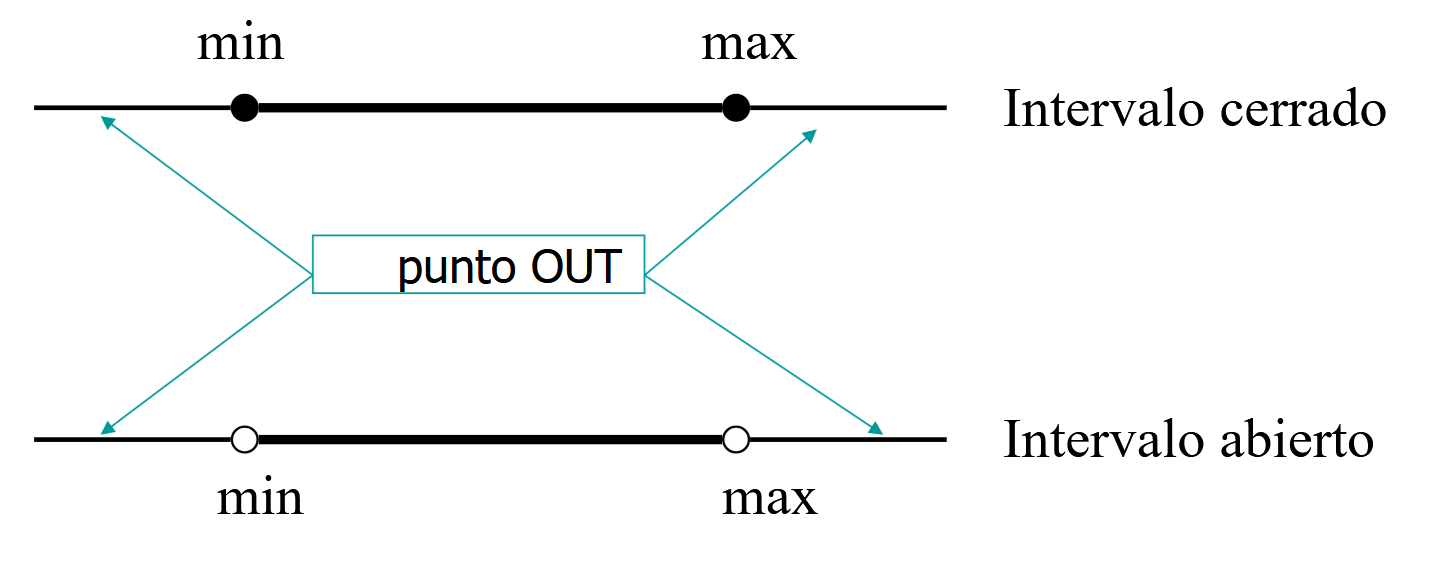
\includegraphics[width=0.45\columnwidth]{images/05/puntoOUT.png}
   \caption{puntoINOUT}
   \label{fig:05/puntoINOUT}
\end{figure}
\begin{figure}[htbp]
   \centering
   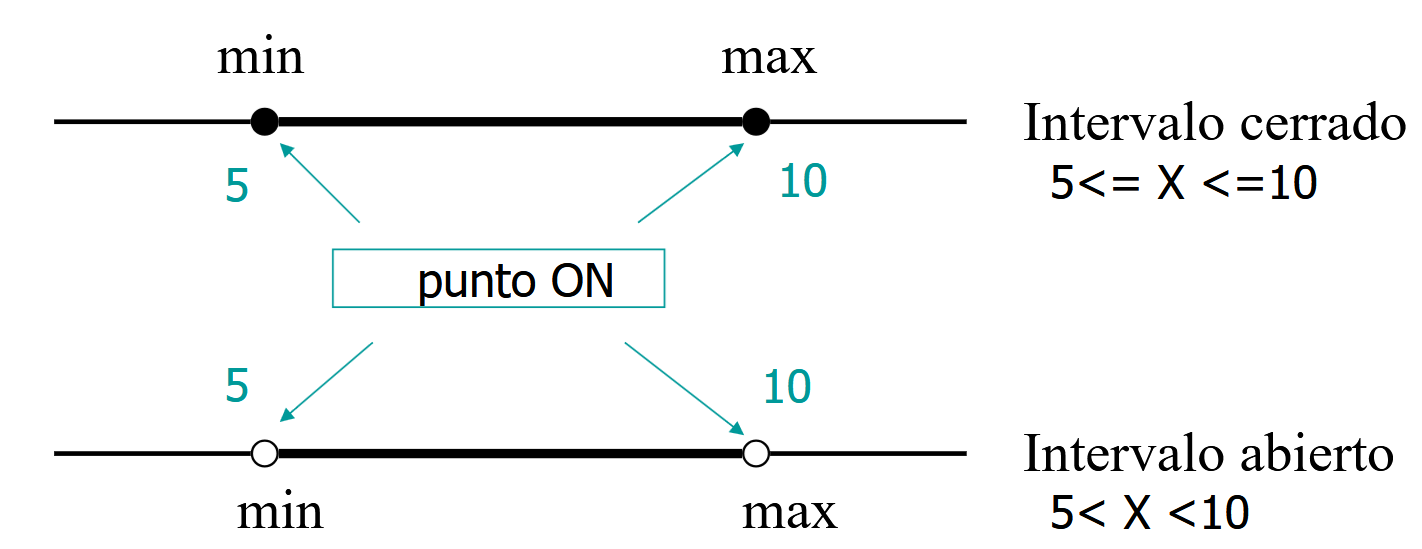
\includegraphics[width=0.45\columnwidth]{images/05/puntoON.png}
   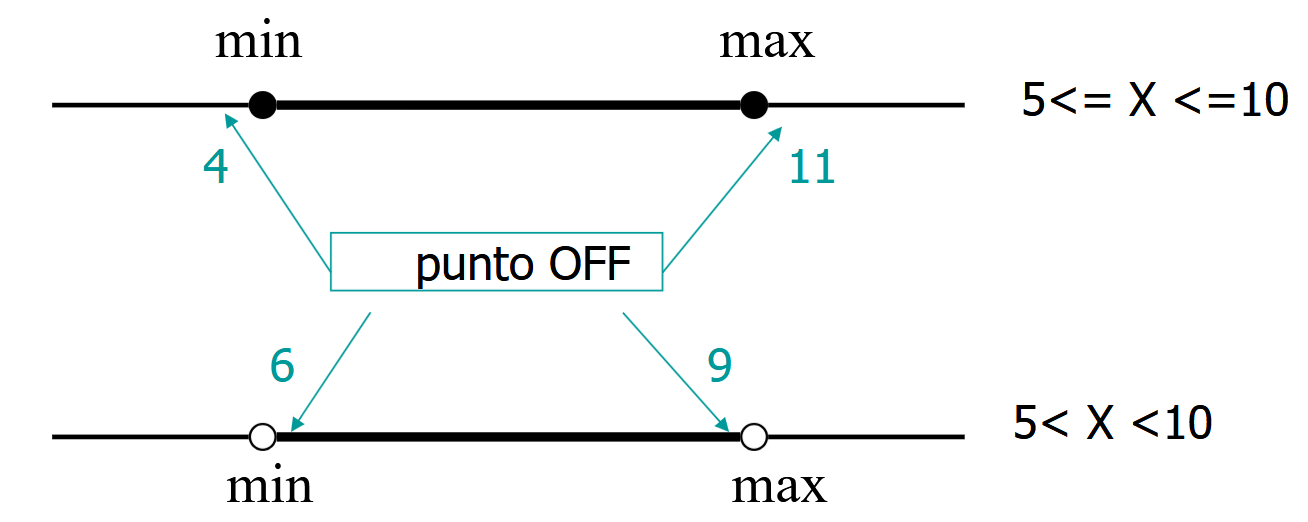
\includegraphics[width=0.45\columnwidth]{images/05/puntoOFF.png}
   \caption{puntoONOFF}
   \label{fig:05/puntoONOFF}
\end{figure}

\begin{itemize}
   \item \textsc{Punto IN} : un punto que pertenece al intervalo
   \item \textsc{Punto OUT} : un punto que no pertenece al intervalo
   \item \textsc{Punto ON} : un punto que pertenece al intervalo y es un límite
   \begin{itemize}
      \item Intervalo cerrado - punto ON satisface la
      condición del intervalo
      \item Intervalo abierto - punto ON \textit{no} satisface la
      condición del intervalo
   \end{itemize}
   \item \textsc{Punto OFF} : un valor cerca del punto límite de un intervalo
   \begin{itemize}
      \item Intervalo cerrado - punto OFF \textit{no} satisface la
      condición del intervalo
      \item Intervalo abierto - punto OFF satisface la
      condición del intervalo
   \end{itemize}
\end{itemize}

La estrategia para diseñar las pruebas de valores límites es 1 punto ON + 1 punto OFF para cada desigualdad de límite.

\begin{paracol}{2}
   \note{Ejemplos:
   \begin{itemize}
      \item 3 <= extras < 10
            \begin{itemize}
               \item Puntos ON: extras = 3; extras = 10
               \item Puntos OFF: extras = 2; extras = 9
            \end{itemize}
      \item 2000 < precio\_base <= 5000
            \begin{itemize}
               \item Puntos ON?
               \item Puntos OFF?
            \end{itemize}
   \end{itemize}}
   
   \switchcolumn
   
   \note{
      \begin{itemize}
         \item $x > 0$ ($x$ es número natural)
               \begin{itemize}
                  \item ON = 0
                  \item OFF = 1
               \end{itemize}
         \item $x \leq 10$ ($x$ es número natural)
               \begin{itemize}
                  \item ON = 10
                  \item OFF = 11
               \end{itemize}
         \item $x > 0$ ($x$ es número real)
               \begin{itemize}
                  \item ON = 0
                  \item OFF = 0,00001
               \end{itemize}
         \item $x \leq 10$ ($x$ es número real)
               \begin{itemize}
                  \item ON = 10
                  \item OFF = 10,0001
               \end{itemize}
      \end{itemize}
   }
\end{paracol}

\section{Matriz del testeo de dominio}
\begin{paracol}{2}
   
   \begin{figure}[htbp]
      \centering
      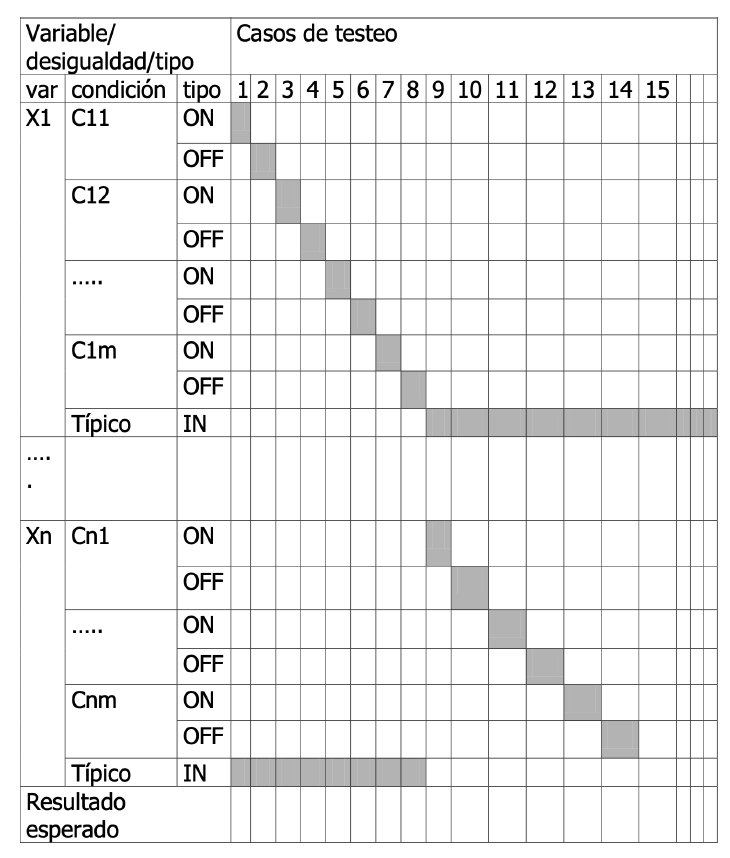
\includegraphics[width=0.70\columnwidth]{images/05/matrizTesteo.png}
      \caption{Matriz de testeo de dominio}
      \label{fig:05/matrizTesteo}
   \end{figure}

   \switchcolumn  

   \colfill

   Una representación conveniente para representar el conjunto de casos de test desarrollados con el testeo de dominio.\\\
   Cada columna es un caso de test.\\
   Cada caso de test:
   \begin{itemize}
   	\item un ON o OFF para la variable en cuestión (diagonal)
   	\item para las demás variables un IN (horizontales)
   \end{itemize}
   \nl

   Tipos de datos ``nonscalar'' no tienen orden, por ejemplo strings, boolean o enumeraciones.
   Los límites del dominio son cerrados y binarios: la variable cumple la condición o no. Entonces,
      \begin{itemize}
      	\item El Punto ON es valor que cumple la condición
      	\item El Punto OFF es valor que no cumple la condición
      \end{itemize}
   \colfill
\end{paracol}

\newpage
\subsection{Money class ejemplo}

\begin{paracol}{2}
   \begin{lstlisting}
class Money {
   private int fAmount;
   private String fCurrency;

   public Money(int amount, String currency) {
      fAmount = amount;
      fCurrency = currency;
   }

   public int amount() {
      return fAmount;
   }

   public String currency() {
      return fCurrency;
   }
}
   \end{lstlisting}

   \switchcolumn

   Imagina que tenemos que testear un componente:
\begin{itemize}
	\item entrada un objeto \lstinline|Money m|
	\item el componente espera que
	\begin{itemize}
      \item \lstinline|m.amount() >= 0|
      \item \lstinline|m.currency()| in \lstinline|{EURO,USD, GBP, YEN}|
   \end{itemize}
	\item Si el cliente quiere pagar en \lstinline|USD,GBP o YEN|, tiene que pagar \lstinline|10%| de costes de administración
	\item Si el cliente paga en \lstinline|EURO|, no hay costes de administración
\end{itemize}
\end{paracol}

\begin{figure}[htbp]
   \centering
   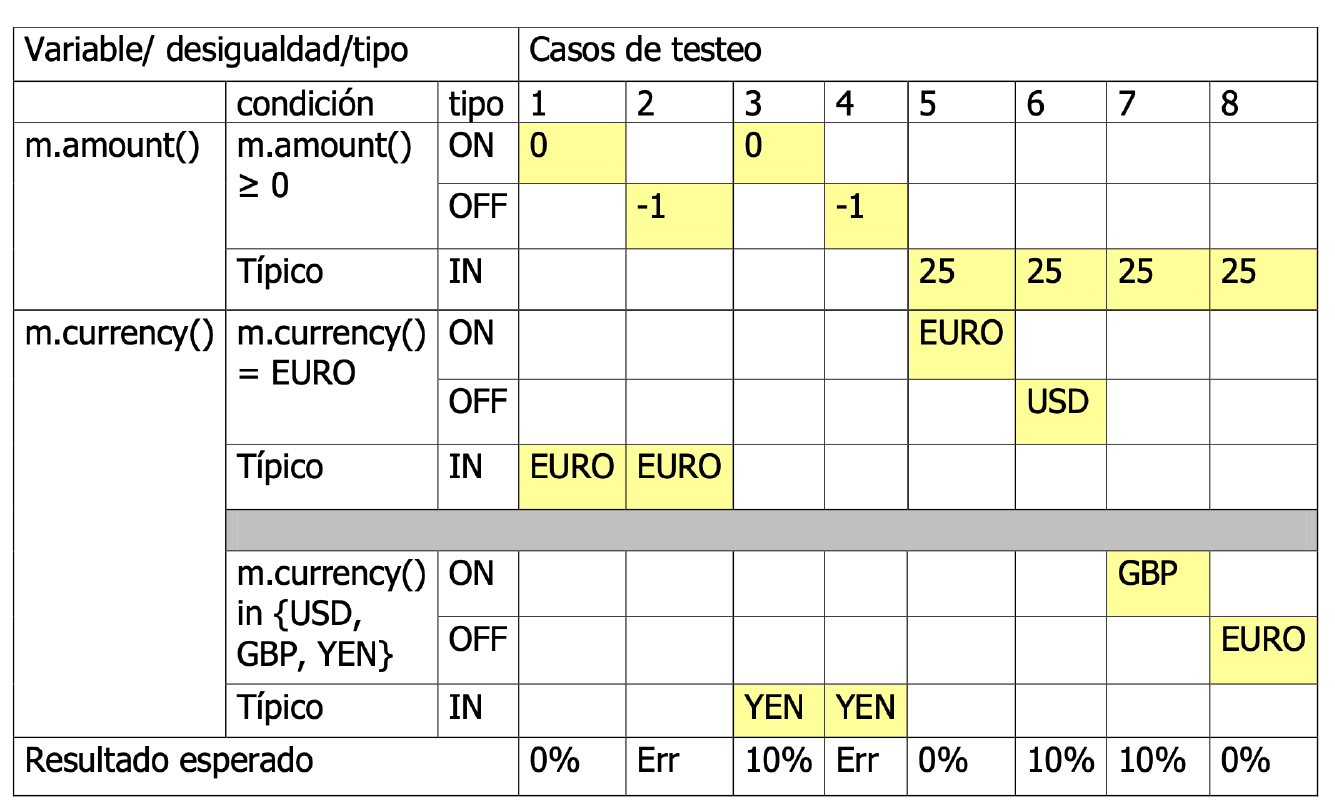
\includegraphics{images/05/matrizMoney.png}
   \caption{Matriz de testeo de dominio para la clase Money}
   \label{fig:05/matrizMoney}
\end{figure}

Si tenemos una clase compleja que no se puede tratar como un escalar, es posible que podemos utilizar una ``abstración de estados'' para definir los límites del dominio.
Por ejemplo considera una clase \lstinline|Pila| (\textit{stack}), que se puede encontrar en tres estados:
\begin{enumerate}
   \item vacío - \lstinline|stack.size() == 0|
   \item cargado - \lstinline|stack.size() > 0 && stack.size < MAXSTACK|
   \item lleno - \lstinline|stack.size() == MAXSTACK|
\end{enumerate}

\begin{itemize}
   \item Punto ON / vacío - \lstinline|stack.size() == 0|
   \item Punto IN / vacío - \lstinline|stack.size() == 0|
   \item Punto OFF / vacío - \lstinline|stack.size() == 1|
   \item Punto ON / cargado - \lstinline|stack.size() == MAXSTACK - 1|
   \item Punto IN / cargado - \lstinline|stack.size() == ceiling(MAXSTACK / 2) |
   \item Punto OFF / cargado - \lstinline{stack.size() == 0 || MAXSTACK}
   \item Punto ON / lleno - \lstinline|stack.size() == MAXSTACK|
   \item Punto IN / lleno - \lstinline|stack.size() == MAXSTACK|
   \item Punto OFF / lleno - \lstinline|stack.size() == MAXSTACK + 1|
\end{itemize}

\section{Máquinas de estado}

La idea es modelar el comportamiento del sistema como una
máquina de estados.
Los casos de prueba diseñados con esta técnica tratarán de
cubrir los diferentes estados y transiciones especificados en la
máquina de estados que representa el sistema.

\begin{figure}[htbp]
   \centering
\begin{tikzpicture}[
   node distance=6cm,
   state/.style={
      rectangle, 
      rounded corners=15pt, 
      draw=cyan!40, 
      fill=cyan!5, 
      very thick, 
      minimum height=2cm, 
      minimum width=6cm,
      font=\large,
      align=center
      },
      transition/.style={
         ->, 
         >=stealth, 
         %  shorten >=1pt, 
         %  shorten <=1pt, 
         very thick
         }
         ]
         % Stati
         \node[state] (s1) {\textit{\footnotesize(S1)}\\[0.2cm] Bombilla Encendida};
         \node[state] (s2) [below=3cm of s1] {\textit{\footnotesize(S2)}\\[0.2cm] Bombilla Apagada};
         
         % Transizioni
         % Prima transizione spostata più a destra
         \draw[transition] (s1.south west) to[out=-135, in=135] node[left, align=center, font=\itshape] {presionar interruptor} (s2.north west);
         
         % Seconda transizione (invariata)
         \draw[transition] (s2.north east) to[out=45, in=-45] node[right, align=center, font=\itshape] {[hay electricidad]\\presionar interruptor} (s1.south east);
         
         % Terza transizione (self-loop) spostata più a destra
         \draw[transition] (s2.240) to[out=-120, in=-60, looseness=3] 
         node[below, align=center, font=\itshape] {[no hay electricidad]\\presionar interruptor} 
         (s2.310);
      \end{tikzpicture}
      \caption{Ejemplo de máquina de estados}
      \label{fig:05/maquinaEstado}
   \end{figure}


\begin{table}[htbp]
   \centering
   \setlength{\tabcolsep}{10pt} % Default value: 6pt
   \renewcommand{\arraystretch}{1.5} % Default value: 1
   \begin{tabular}{|r|r|r|r|}
      \hline
      Test case&     1        &     2                    &     3  \\ \hline
      \textbf{Estado inicial} & S1 - Encendida           & S2 - Apagada          & S2 - Apagada \\ \hline
      \textbf{Entrada}        & Presionar interruptor    & Presionar interruptor & Presionar interruptor \\ \hline
      \textbf{Condición}      & Hay electricidad         & Hay electricidad   & No hay electricidad \\ \hline
      \textbf{Estado final}   & S2 - Apagada             & S1 - Encendida        & S2 - Apagada  \\ \hline
      \end{tabular}
   \caption{Tabla de ejemplo para la máquina de estados de luz con interruptor}
   \label{tab:05/maquinaEstado}
\end{table}
\labelitemize{Cobertura}{
   \begin{itemize}
      \item Cobertura de \textbf{estados}: Este criterio se satisface cuando los casos de prueba recorren todos los estados.
      \note{
         Test case: 2
      }
      \item Cobertura de \textbf{transiciones}: En este caso, se satisface el criterio cuando se recorren todas las transiciones.
      \note{
         Test case: 1,2,3
      }
      \item Cobertura de \textbf{pares de transiciones}: Para cada estado se cubren las combinaciones de transiciones de entrada y salida.
      \note{
         Test case: 1,2,3
      }
   \end{itemize}
}

Cobertura de estados: 2
Cobertura de transiciones: 1, 2 y 3.
Cobertura pares de transiciones: 1, 2 y 3